\subsection{Research Thrust 1: Modeling driver behavior, and emotions}
\label{sec:behaviour}

 %The ability to (1) detect, (2) assess and (3) manage a person’s emotions has been identified to be the predictor of success in relating to the people around us. 
 Being able to read other’s emotional cues not only allows us to understand how people are feeling at a given time, but it also helps us to predict how they will respond in different scenarios. 
 If an autonomous vehicle can detect the emotional cues of the driver, and more importantly respond to them, then it can develop ``human-like'' trust with the driver.
 Research suggests that emotions are normally associated with specific events or occurrences \cite{cowie2001emotion}, and they can significantly influence our thoughts and behaviors. 
 %Additionally, we can use reason to evaluate our emotions, interpret them, and reassess our initial reactions to them. 
 %Therefore, by detecting certain events and occurrences, we may be able to assess and predict individual emotional states and use reason to soften their impact or ``shift'' their meaning. 
 This research thrust aims to enhance driver experience, safety, and trust in the AV. 
 We do so by automatically and accurately detecting, assessing, and managing the passengers behaviors and emotions. 
 
Several Naturalistic Driving Studies (NDS) have studied human behavior in vehicles in different safety-related conditions, with the specific emphasis towards crash or near-crash incidents. 
In these studies, cars were equipped with sensors and devices that continuously monitor various aspects of driving behavior such as vehicle acceleration, deceleration, location, and speed, driver-related information such as eye, head and hand movement, and environmental conditions such as traffic and weather conditions \cite{eenink2014udrive, simons2015naturalistic, fridman2017autonomous, klauer2006impact, victor2015analysis, papazikou2017detecting}. 
For instance, in \cite{eenink2014udrive} researchers identified that certain driver-personality traits are prone to committing speeding violations; 
or bad behaviors may cluster together, where drivers who perform one type of risky behavior are more likely to engage in other types of risky behaviors. \begin{figure}
    \centering
    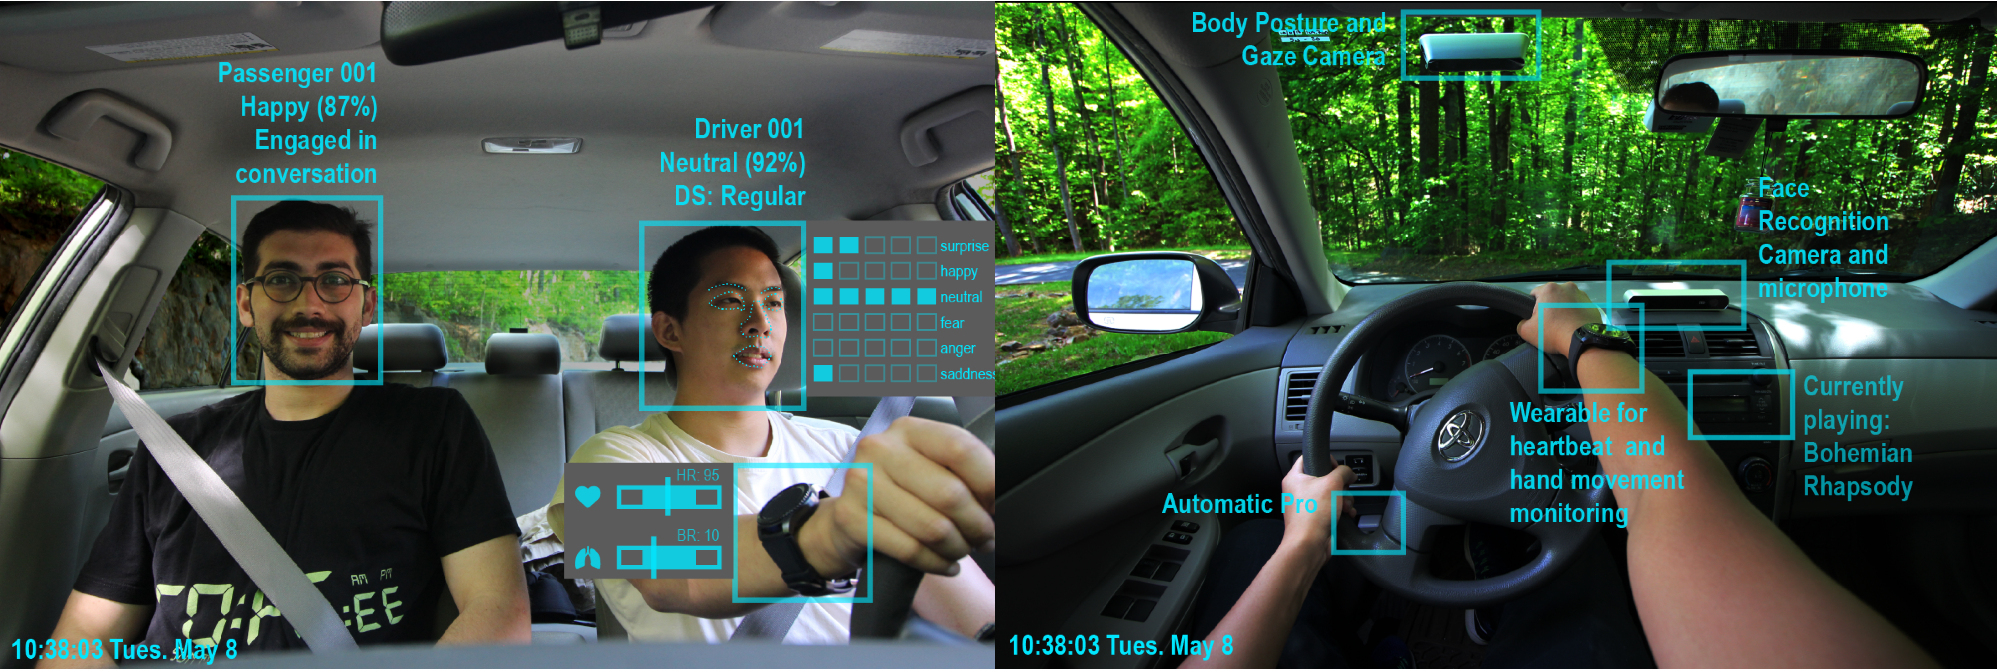
\includegraphics[width=0.8\columnwidth]{figures/car.pdf}
    \caption{Overview of instrumentation of vehicles and the collected information from participants}
    \label{fig:sensors}
\end{figure}
Although these studies provide significant insights on the driver behavior in different scenarios and contextual settings, they specifically focus only on safety-related behaviors that result in crashes or near-crash incidents; 
%additionally, the first generation of NDS used manual video annotation techniques to identify driver behaviors in specific epochs of driving (CITE), which requires extensive time and manpower to complete. 
Due to complexities related to human behaviors (i.e., dynamic changes in human behaviors) many of the NDS were limited to short-term monitoring and as a result, lacked in identifying how the driver behaviors may change based on various contextual, environmental, and social settings. 
%With the growing interest in long-term behavioral monitoring and automated monitoring approaches, in more recent NDS studies, researchers are focusing on large-scale computer vision-based and audio processing analyses of human behavior where information can  semi-automatically and/or automatically be extracted from raw video and audio feeds (CITE). 
In a recent study researchers are using computer vision and voice-processing techniques to monitor drivers body posture, eye movement, and emotions to predict driver's frustration and gaze region that may result in unsafe behaviors while driving semi-automated and fully-automated vehicles \cite{fridman2017autonomous, abdic2016driver, fridman2016driver, fridman2018cognitive, fridman2016owl}. 
  
At higher levels of autonomy, behavioral and emotional information not only are extremely useful for increasing safety of AVs, they can also be applied towards optimizing control actions of AVs, and most importantly, enhancing the  driving-experience for the driver and/or passenger(s); for instance, by identifying that the driver is feeling ``happy'', AVs can optimize their route selection in order to increase the drivers positive emotions, potentially enhancing the driver's mental health. 
Additionally, by optimizing the decision making of automated systems around the user's specific preferential and comfort profiles, research suggests that the automated system can better gain user trust \cite{mouloua2018automation, noah2017first}. 
%Although the more recent NDS are implementing automated monitoring techniques for detecting driver behaviors and emotions, they specifically focus on identifying safety-related behaviors in semi and fully-automated vehicles. 
There exists a lack of understanding on the causation of behaviors as a result of environmental, emotional, physiological, and social factors. %(\textit{problem 1}); and integration of behavioral models into AV safety and control actions(\textit{ problem 2}). 
%Additionally, within the exiting work, limited number of studies have investigated the impacts of social interactions on the driver and passengers behaviors and emotions; by being able to identify the impacts of social interactions on certain behaviors, AVs can better optimize the vehicle's level of autonomy according to the behavioral and emotional states of the driver as well. 
%current studies also lack real-time data processing.
In this research thrust, we aim to understand how environmental, physiological, and social factors may influence and/or cause certain behaviors and emotions in the driver and passengers. 
When we break down this hypothesis further, the following are the questions of interest:
\begin{enumerate}[itemsep=0pt,parsep=0pt,topsep=4pt,leftmargin=0.4in]
    \item What is the taxonomy of driving behaviors and emotions based on environmental conditions, social interactions, and physiological changes?
    \item How can driving behavior and emotions be non-intrusively and with least number of sensors be detected?
    \item Do people have differentiating “trust” profiles according to specific behaviors and contextual conditions?  
\end{enumerate}

While existing literature has considered each of the environmental, social, and physiological factors separately, the challenge lies in learning causal relationships between these factos, and how they influence emotion and behaviors of the drivers.  
Specifically, we will gather data and build models for (1) factors that influence specific human emotions and (2) the downstream consequences of particular emotions on their behaviors. 
For instance, we will gather data to asses what environmental (e.g., weather, thermal conditions, lighting, noise) and social factors (e.g., social interaction), physiological factors (e.g.,arm movement) trigger particular emotions. 
One outcome of this work will also be able to develop a library of emotions, behaviors, social interactions, and environmental changes. 
Our preliminary investigations have revealed the following taxonomy for driver behaviors:

\noindent[\textbf{Risky driving}] is often addressed as one of the caveats of autonomous vehicles. For example, if drivers sufficiently trust vehicles, some drivers will likely follow the front car closely or drive faster than usual. 

\noindent[\textbf{Anxious driving}] style. To better understand this anxious drivers, we need to look at the plausible sources of anxiety regarding autonomous vehicles. On one hand, people can be anxious about their poor driving skill. Fully automated vehicles can solve this issue. On the other hand, people can be anxious about not being able to control over something. In this case, we can design the interface so that drivers can make the driver feel more in control.

\noindent[\textbf{Dissociated driving}] includes errors and mistakes (e.g., errors in gear shift or lights). If this stems from poor (or inexperienced) driving, again fully autonomous vehicles can solve this issue. Drivers do not need to differentiate gear shifts or calculate route themselves. However, detecting the casual effects of dissociated driving and being able to predict this behavior profile remains an open challenge.


\noindent[\textbf{Careful driving}] is referred to ``better safe than sorry''. 
To fulfill this type of drivers' motivation with any type of autonomous vehicles, we can provide more effective and robust monitoring interfaces rather than providing a number of distracting tasks. Such drivers likely want to have higher situation awareness and will be satisfied with the more completed monitoring mechanisms.

We plan to gather the required data both through high fidelity simulations on a full scale diving simulator (Section~\ref{sec:experiment}) and by instrumenting participant-owned vehicles, we will collect and analyze the impact of different factors on driver/passenger behaviors and emotions.
To collect environmental-related information, Automatic Pro will be used to monitor the car's speed and location. 
Automatic Pro will be also used to collect behavioral information such as driver's acceleration and deceleration rates
%(previous research suggests acceleration/deceleration can be used to identify risky or frustrated drivers (CITE)). 
Cameras will be used to capture outdoor conditions such as traffic, weather, pedestrians, signs etc. as well as indoor conditions such as social interactions, drivers and passenger(s)'s body posture, face, head and hand/arm movement. 
Ambient-condition sensors will be used to measure thermal settings, indoor and outdoor noise levels, and lighting levels. 
Audio recorders will be used to capture social interactions as well as any other audio sources (i.e., music, radio, audio books, etc.). 
Wearables such as Samsung Gear or Fitbit will be used to measure the driver and passengers physiological data (i.e., heart rate and hand/arm movement). Through face recognition software (i.e., iMotion, Google API) recorded videos will be processed to create a time-stamped emotional states for the driver and passengers; 
%additionally, audio data will be processed through speech-to-tech and natural language processing techniques to identify and classify various social interactions and audio sources (e.g., music or radio). 
The audio information as well as physiological information can also be used to identify the driver/passengers emotional states. 
Figure~\ref{fig:sensors} provides an overview of the sensors and data that will be collected from the drivers and passenger(s).   


%As it may be difficult to often identify triggers to particular emotions (i.e., passenger may appear already experiencing a particular emotion), we plan to evaluate which environmental (indoor and outdoor) and social factors may be used as cues for particular emotions and/or behaviors. 
%For example, as our preliminary data indicates, in rainy conditions, a driver focuses more on his driving, and as a result his acceleration/declaration rates are dropped compared to normal conditions; meanwhile the driver is more likely to not listen to any music. With this information, we will then assess if we can reliably predict particular emotions or behaviors, given specific contextual, environmental or social factor(s); for instance in a rainy condition, the driver will have higher control of the vehicle.The specific research questions that will be addressed through this approach include: 
By having an understanding about the causation of certain behaviors and emotions, behavioral and emotional models can be developed and integrated into AVs systems where they can optimize the control actions as well as feedback/communication strategies.
%based on the driver preferences and behaviors. 
We will utilize data-driven algorithms that aggregate the information extracted from vision and audio with physiological and environmental information. Through clustering techniques and machine learning algorithms (i.e., CNL and HMM), we will define the behavioral models described above, as a function of emotional traits, environmental conditions, social interactions, and physiological measures.%Madhur to improve
The resulting behavior models will be passed on as a driver profile/preference input to the trajectory planning module of the autonomous vehicle in Thrust 2 (Section~\ref{sec:reachability}), and also to trigger a natural language explanation for the car's actions according to Thrust 3 (Section~\ref{sec:feedback})
While we will largely rely on exiting data-driven and machine learning models and techniques for individual factors modeling and classification, the novelty of this human factors research lies in establishing causal relationships between environmental, emotional, social, and physiological data and driving behavior, and to be able to predict and/or classify driver behavior in real time as an input to the autonomous driving and feedback system.




 

 
 


%\begin{center}
    %\begin{tabular}{ | l | l | l |}
    %\hline
    %Type &  Factors & Sensor/Algorithms \\ \hline
    %\multirow{5}{*}{Environmental Sensing} & Speed & Automatic Pro \\
        %& Location & GPS/Automatic Pro \\
       % & indoor and outdoor conditions & cameras \\
      %  & Passengers' identity and count & cameras \\
     %   & Weather Conditions & Camera and weather database\\\hline
    %\multirow{8}{*}{Human Sensing} & Face features & eye tracking, camera, facial recognition \\
       % & Noise levels & noise-level sensors \\
       % & Passenger voice & Voice recorder, Natural Language Processing \\
      %  & Brake and acceleration rate & Automatic Pro \\
     %   & Grip on steering wheel & pressure sensor \\
    %    & Music and other social media use & APIs (e.g., Spotify) \\
   %     & Social interaction & Camera and voice recorder \\ \hline
  %  
 %   \end{tabular}
%\end{center}








